\section{Instruction Fetch}
The purpose of this unit is to:
\begin{itemize}
	\item hold the current value of the program counter (\texttt{PC}); 
	\item increment it when executing sequential code;
	\item fetch the next instruction from instruction memory
\end{itemize}

\subsection{Structure} A RTL description would contain a \texttt{PC} register, treated as a special register within the processor and an incrementer to compute \texttt{PC+4}. Normally, the PC is updated with the next sequential address. However, when a jump occurs, a selection logic driven by the control unit inside the ID stage causes the PC to be updated using an address coming from a dedicated adder that computes the target address for jumps or branches. In the case of a stall, the PC is not updated at all and the same instruction is refetched from memory.

This stage reads from the instruction memory, requiring a 32-bit output port to deliver the desired address and a 32-bit input port to receive the instruction word. 

\autoref{fig:ifstage} shows an high-level representation of this part of the processor. The \texttt{stall} and \texttt{jump} signals are provided by the control unit and cross the stage boundary. The loop involving the jump address calculation with the dedicated adder in the ID stage and the selection logic in this stage is potentially a critical path and it crosses the pipeline boundaries. However, we will see that the path including the main adder in the execution stage is way longer.

\begin{figure}[h]
	\centering
	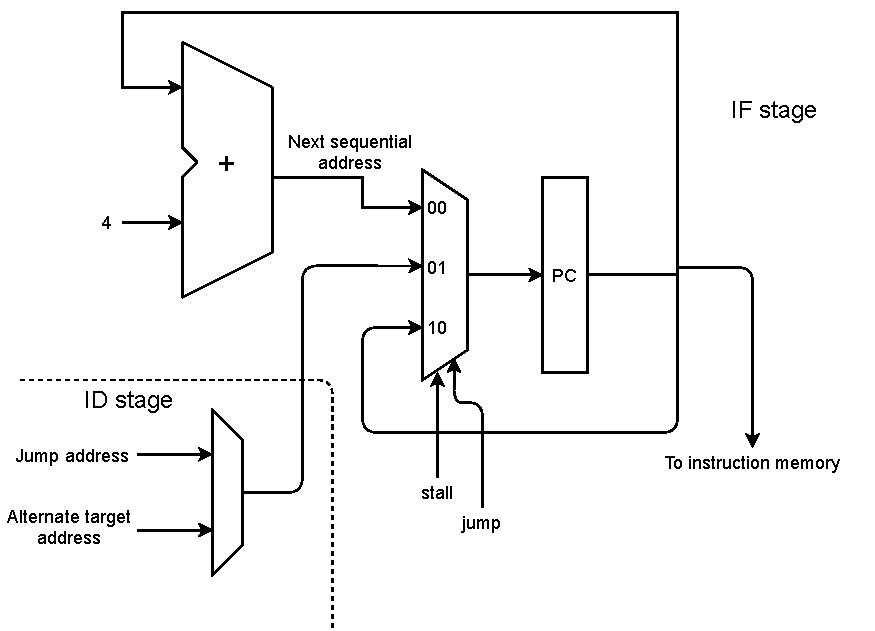
\includegraphics[width=0.6\textwidth]{../images/IF.pdf}
	\caption{RTL schematic of the instruction fetch stage, with part of the ID stage reported which selects the right jump address according to whether it is triggered by a jump instruction or a misprediction.}
	\label{fig:ifstage}
\end{figure}